% generated by scripts/pkl_to_latex.py
% source PKL : uscan_v1_L6_Ne6_t1_mode-uniform_nmin2_solver-gcg_sz0_restarts10_iter200_kmax4_tol1em09_U1to20_N20-d03a74da789e.pkl
% scan type  : uscan
% state      : gs
% quantity   : purity
% requires   : \usepackage{pgfplots} \pgfplotsset{compat=1.18}
% colours match the matplotlib PDF (tab10 cycle)
\definecolor{gmeC0}{HTML}{1F77B4}
\definecolor{gmeC1}{HTML}{FF7F0E}
\definecolor{gmeC2}{HTML}{2CA02C}
\definecolor{gmeC3}{HTML}{D62728}
\definecolor{gmeC4}{HTML}{9467BD}
\definecolor{gmeC5}{HTML}{8C564B}
\definecolor{gmeC6}{HTML}{E377C2}
\definecolor{gmeC7}{HTML}{17BECF}

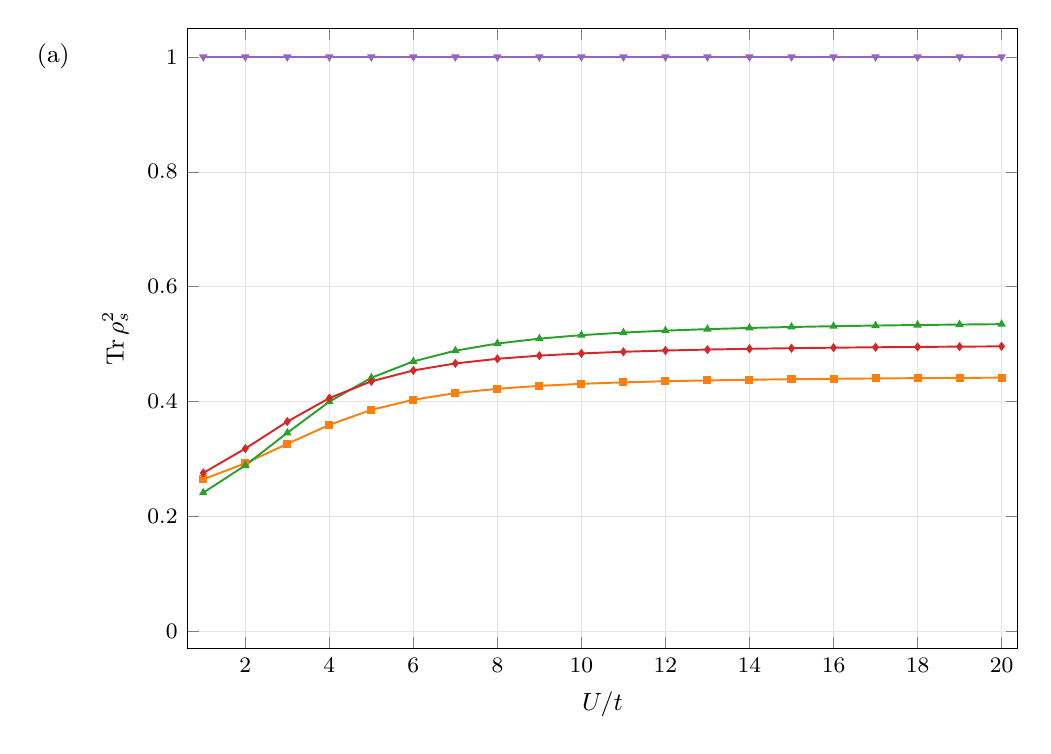
\begin{tikzpicture}
  \begin{axis}[
    width=\columnwidth,
    height=0.78\columnwidth,
    xlabel={$U/t$},
    ylabel={$\mathrm{Tr}\,\rho_s^2$},
    grid=both,
    grid style={line width=.1pt, draw=gray!20},
    tick label style={font=\footnotesize\rmfamily, /pgf/number format/fixed},
    label style={font=\small\rmfamily},
    scaled ticks=false,
    legend style={font=\scriptsize\rmfamily, draw=gray!40, at={(0.5,1.03)}, anchor=south, /tikz/every even column/.append style={column sep=6pt}},
    legend cell align={left},
    legend columns=2,
    ymin=-0.03,
    ymax=1.05,
    xmin=0.62,
    xmax=20.38,
    after end axis/.append code={\node[anchor=east, font=\small\rmfamily] at (axis description cs:-0.13,0.954) {(a)};},
  ]
    \addplot[color=gmeC1, mark=square*, mark size=1.1pt, line width=0.7pt] coordinates {
        (1,0.264586) (2,0.292312) (3,0.32617) (4,0.359322)
        (5,0.38535) (6,0.403097) (7,0.414607) (8,0.422126)
        (9,0.427193) (10,0.430737) (11,0.433303) (12,0.435219)
        (13,0.436688) (14,0.437839) (15,0.438759) (16,0.439507)
        (17,0.440122) (18,0.440635) (19,0.441067) (20,0.441435)
    };
    \addplot[color=gmeC2, mark=triangle*, mark size=1.1pt, line width=0.7pt] coordinates {
        (1,0.24117) (2,0.288688) (3,0.345463) (4,0.399589)
        (5,0.441352) (6,0.469801) (7,0.488477) (8,0.5009)
        (9,0.509436) (10,0.515511) (11,0.519979) (12,0.52336)
        (13,0.525979) (14,0.528051) (15,0.529718) (16,0.531081)
        (17,0.532209) (18,0.533153) (19,0.533952) (20,0.534634)
    };
    \addplot[color=gmeC3, mark=diamond*, mark size=1.1pt, line width=0.7pt] coordinates {
        (1,0.275557) (2,0.317989) (3,0.364999) (4,0.405812)
        (5,0.435041) (6,0.454068) (7,0.466268) (8,0.474296)
        (9,0.479785) (10,0.483685) (11,0.486551) (12,0.488719)
        (13,0.490399) (14,0.491728) (15,0.492798) (16,0.493672)
        (17,0.494395) (18,0.495001) (19,0.495513) (20,0.495951)
    };
    \addplot[color=gmeC4, mark=triangle*, mark size=1.1pt, mark options={rotate=180}, line width=0.7pt] coordinates {
        (1,1) (2,1) (3,1) (4,1)
        (5,1) (6,1) (7,1) (8,1)
        (9,1) (10,1) (11,1) (12,1)
        (13,1) (14,1) (15,1) (16,1)
        (17,1) (18,1) (19,1) (20,1)
    };
  \end{axis}
\end{tikzpicture}
